\documentclass{article}
\usepackage{tikz}

\begin{document}

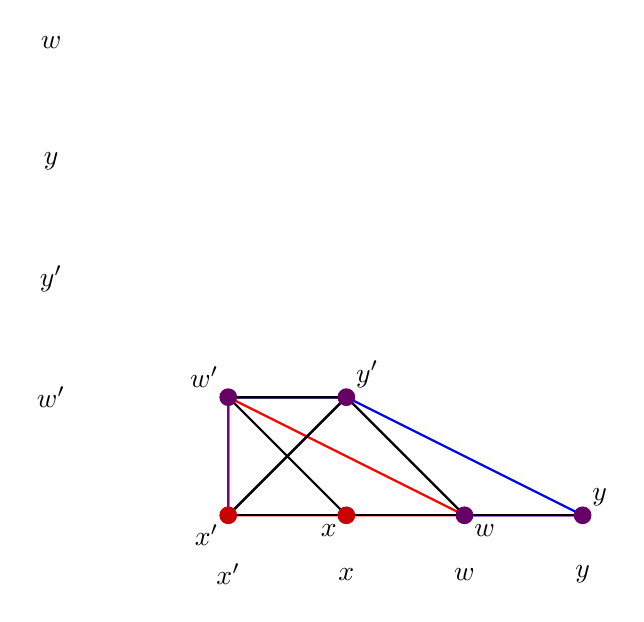
\begin{tikzpicture}[scale=1.5]
    % Define coordinates for the vertices
    \coordinate (w) at (3,0);
    \coordinate (y) at (4,0);
    \coordinate (x) at (2,0);
    \coordinate (x') at (1,0);
    \coordinate (w') at (1,1);
    \coordinate (y') at (2,1);

    % Draw the edges of the graph
    \draw[thick, color=red] (x') -- (x) -- (y) -- (w) -- (w') -- (x');
    \draw[thick, color=blue] (w') -- (y') -- (y) -- (w);
    \draw[thick, color=violet] (w') -- (y') -- (x') -- (w');

    % Draw the edges connecting the vertices
    \draw[thick, color=black] (x') -- (y') -- (w') -- (x);
    \draw[thick, color=black] (x') -- (y) -- (w) -- (x');
    \draw[thick, color=black] (w') -- (y') -- (w) -- (y');

    % Draw the vertices
    \filldraw[fill=violet!80!black, draw=violet!80!black] (w') circle (2pt) node[above left] {$w'$};
    \filldraw[fill=violet!80!black, draw=violet!80!black] (y') circle (2pt) node[above right] {$y'$};
    \filldraw[fill=violet!80!black, draw=violet!80!black] (y) circle (2pt) node[above right] {$y$};
    \filldraw[fill=violet!80!black, draw=violet!80!black] (w) circle (2pt) node[below right] {$w$};
    \filldraw[fill=red!80!black, draw=red!80!black] (x') circle (2pt) node[below left] {$x'$};
    \filldraw[fill=red!80!black, draw=red!80!black] (x) circle (2pt) node[below left] {$x$};

    % Label the vertices
    \node at (1,-0.5) {$x'$};
    \node at (2,-0.5) {$x$};
    \node at (3,-0.5) {$w$};
    \node at (4,-0.5) {$y$};
    \node at (-0.5,1) {$w'$};
    \node at (-0.5,2) {$y'$};
    \node at (-0.5,3) {$y$};
    \node at (-0.5,4) {$w$};
\end{tikzpicture}

\end{document}